\section{Die Brownsche Bewegung}

Oft wird die Brownsche Bewegung (oder auch Wiener Prozess) axiomatisch definiert. In dieser Arbeit werden 
direkt kumulative Summen von Normalverteilungen betrachtet. Zuerst wird eine vereinfachte Darstellung des Prozesses eingeführt, 
die diskrete Brownsche Bewegung. Die Argumentation ist angelehnt an Behrends \cite{behrends} (2013, Kap. 5).

\subsection{Diskrete Brownsche Bewegung}

\begin{defi}[Diskrete Brownsche Bewegung]
Die elementare Brownsche Bewegung sei ein stochastischer Prozess, 
der aus einer Folge von Zufallsvariablen $\xi_n, n \in \Bbb N_0$ besteht, wobei
$$\xi_n = \sum_{i=1}^n \eta_i, \quad \eta_i \sim N(0,1)$$. 
Die Zufallsvariablen $\eta_i$ sind unabhängig und identisch verteilt. Nun 
Nun wird eine stetige Zeitentwicklung durch lineare Interpolation eingeführt:
$$b^{(1)}(t) := \xi_{\lfloor t \rfloor} + (t - \lfloor t \rfloor)(\xi_{\lfloor t \rfloor + 1} - \xi_{\lfloor t \rfloor}), \quad t \geq 0.$$
Die Funktion $b^{(1)}(t)$ wird diskrete Brownsche Bewegung erster Ordnung genannt.
Der Name rührt daher, dass in eine Zeiteinheit genau eine Normalverteilung einbezogen wird.
Im Allgemeinen wird die diskrete Brownsche Bewegung $b^{(N)}(t)$ $N$-ter Ordnung definiert als
$$b^{(N)}(t) := \frac{1}{\sqrt{N}} \left ( \xi_{\lfloor Nt \rfloor} + (Nt - \lfloor Nt \rfloor)(\xi_{\lfloor Nt \rfloor + 1} - \xi_{\lfloor Nt \rfloor}) \right ), \quad t \geq 0.$$
Hierbei wird in eine Zeiteinheit $N$ Normalverteilungen einbezogen. Der Faktor $1/\sqrt{N}$ dient dazu, die Varianzen der Normalverteilungen zu normieren.

\end{defi}

\begin{bsp}[Visualisierung der diskreten Brownschen Bewegung]
Das folgende R-Programm (Ausschnitt) generiert eine diskrete Brownsche Bewegung N-ter Ordnung.

\begin{lstlisting}
  n_points <- N * T_max
  eta <- rnorm(n_points, mean=0, sd=1)
  xi <- c(0, cumsum(eta))
  t_grid <- seq(0, T_max, length.out=steps)
  k <- floor(N * t_grid)
  frac <- N * t_grid - k
  vals <- xi[k+1] + frac * (xi[k+2] - xi[k+1])
  vals <- vals / sqrt(N)
\end{lstlisting}
Für verschiedene Werte von $N$ ergeben sich die folgenden Grafiken:

\begin{figure}[H]
    \centering
    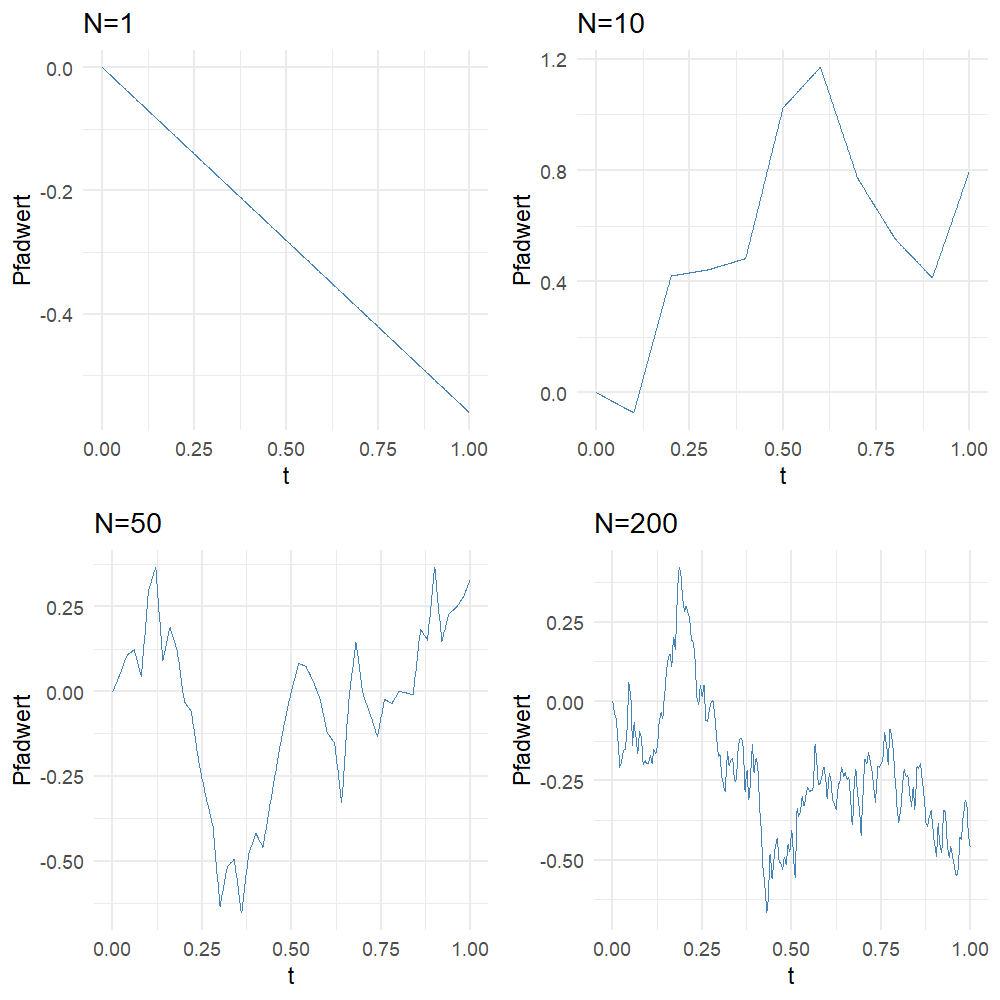
\includegraphics[width=0.9\textwidth]{images/disrete_bb.png}
    \caption{Diskrete Brownsche Bewegung erster, zehnter, fünfzigster und zweihundertster Ordnung}
    \label{fig:brownian}
\end{figure}

\end{bsp}

\begin{lemma}[Martingal-Eigenschaft der diskreten Brownschen Bewegung]
Ohne Beschränkung der Allgemeinheit wird der Fall $N=1$ betrachtet, sonst kann die Zeit skaliert werden.
Ebenso wird nur der Fall $t \in \Bbb N_0$ untersucht: Der Prozess ist also wieder diskret. Das ist
ausreichend, da im Verlauf der Arbeit der Grenzprozess $N \to \infty$ relevant 
wird. Dann ist jeder Wert der Brownschen Bewegung beliebig nah an einem der diskreten Werte, 
und die Martingal-Eigenschaft folgt aus der Stetigkeit des Erwartungswertes. Der stetig interpolierte 
diskrete Prozess an sich ist nämlich kein Martingal. \textit{Beweis.}
Zuerst wird der Fall $m=n+1$ betrachtet: zu zeigen ist
$$E(b^{(1)}(m) | b^{(1)}(n)=v) = v.$$
Da $b^{(1)}(m) = b^{(1)}(n) + \eta_{n+1}$ folgt
$$E(b^{(1)}(m) | b^{(1)}(n)=v) = E(v + \eta_{n+1} | b^{(1)}(n)=v) = v + E(\eta_{n+1}) = v.$$
Nun der allgemeine Fall $m > n+1$: aus dem Satz des iterierten Erwartungswertes folgt
$$E(b^{(1)}(m) | b^{(1)}(n)=v) = E(E(b^{(1)}(m) | b^{(1)}(m-1)) | b^{(1)}(n)=v).$$
Da $E(b^{(1)}(m) | b^{(1)}(m-1)) = b^{(1)}(m-1)$ folgt
$$E(b^{(1)}(m) | b^{(1)}(n)=v) = E(b^{(1)}(m-1) | b^{(1)}(n)=v).$$
Induktiv folgt die Behauptung. \qed \\

\end{lemma}

\begin{lemma}[Varianz der diskreten Brownschen Bewegung]
$$
\begin{aligned}
V(b^{(N)}(t)) &= \frac{1}{N} \left ( V(\xi_{\lfloor Nt \rfloor}) + (Nt - \lfloor Nt \rfloor)^2 \cdot V(\xi_{\lfloor Nt \rfloor + 1} - \xi_{\lfloor Nt \rfloor}) \right ) 
\\ &= \frac{1}{N} (\lfloor Nt \rfloor + (Nt - \lfloor Nt \rfloor)^2)  
\\ &= \frac{\lfloor Nt \rfloor}{N} + \frac{(Nt - \lfloor Nt \rfloor)^2}{N}.
\end{aligned}
$$
Im Grenzübergang $N \to \infty$ konvergiert $\frac{\lfloor Nt \rfloor}{N} \to t$ und $\frac{(Nt - \lfloor Nt \rfloor)^2}{N} \to 0$.
\qed
\end{lemma}

\subsection{Nützliche Ergebnisse aus der Stochastik}
Im Folgenden Beweis zur Stetigkeit der Pfade werden einige Ergebnisse aus der Stochastik verwendet, die hier zusammengefasst, aber nicht bewiesen werden.

\begin{lemma}[Reihenkriterium für fast sichere Konvergenz, Henze \cite{henze} S. 201]
Sei $(X_n)_{n \in \Bbb N}$ eine Folge von Zufallsvariablen. Wenn es eine Reihe $\sum_{n=1}^\infty a_n \lt \infty$ mit $a_n \geq 0$ gibt, so dass
$$P(|X_n| > \varepsilon) \leq a_n \quad \text{für alle } n \in \Bbb N \text{ und jedes } \varepsilon > 0,$$
dann konvergiert $X_n$ fast sicher gegen $0$, d.h.
$$P\left(\lim_{n \to \infty} X_n = 0\right) = 1.$$
Wird hier nicht bewiesen. \qed
\end{lemma}

\begin{satz}[Cramér-Wold-Technik, Henze \cite{henze} S. 225]
Seien $(X_n)_{n \in \Bbb N}$ und $X$ Zufallsvektoren in $\Bbb R^d$. Dann sind folgende Aussagen äquivalent:
\begin{enumerate}
    \item $X_n \xrightarrow{d} X$ für $n \to \infty$.
    \item Für alle $t \in \Bbb R^d$ gilt $t^T X_n \xrightarrow{d} t^T X$ für $n \to \infty$.
\end{enumerate}
Wird hier nicht bewiesen. \qed \\
Die Cramér-Wold-Technik erlaubt es, mehrdimensionale Verteilungskonvergenz auf eindimensionale Berechnungen zurückzuführen.
\end{satz}

\subsection{Die Brownschen Bewegung als Grenzprozess und Eigenschaften}
Nun wird der Grenzprozess $N \to \infty$ betrachtet. Intuitiv wird die Zeit immer feiner aufgelöst,
und es werden immer mehr Normalverteilungen in eine Zeiteinheit einbezogen. Vorerst ist jedoch unklar, 
ob der Grenzprozess überhaupt existiert. Um die Konvergenz des Prozesses zu zeigen, wird die Verteilungskonvergenz 
untersucht. Konvergenz der einzelnen Zeitpunkte (oder endlich-dimensionalen Vektoren) reicht nicht 
für Konvergenz der Prozesse als Funktionen. Dazwischen könten „Spikes“/hochfrequente Oszillationen liegen,
die jede feste endliche Stichprobe verfehlen, aber im Supremumsabstand sichtbar bleiben, zum Beispiel könnte der
Prozess bei irrationalen Zeiten den Wert $\infty$ annehmen (Das ist natürlich nur ein Gedankenexperiment und 
sehr unintuitiv). Daher wird die Konvergenz in 3 Schritten untersucht:
\begin{enumerate}
  \item Verteilungskonvergenz der einzelnen Zeitpunkte
  \item Verteilungskonvergenz von endlich-dimensionalen Vektoren und die Kovarianzen
  \item Stetigkeit der Pfade des Grenzprozesses
\end{enumerate}

\begin{lemma}[Verteilungskonvergenz der diskreten Brownschen Bewegung]
Es existiert ein stochastischer Prozess $W_t, t \geq 0$, so dass für jedes $t$ die Verteilung von $b^{(N)}(t)$ gegen die Verteilung von $W_t$ konvergiert, wenn $N \to \infty$.
\textit{Beweis.}
Da 
$$b^{(N)}(t) = \frac{1}{\sqrt{N}}\big(\xi_k+\alpha(\xi_{k+1}-\xi_k)\big)
=\frac{1}{\sqrt{N}}\big(\xi_k+\alpha\,\eta_{k+1}\big).
$$
ist $b^{(N)}(t)$ eine lineare Kombination von Normalverteilungen, und daher widerum 
normalverteilt. Erwartungswert und Varianz wurden bereits berechnet:
$$
E(b^{(N)}(t)) = 0, \quad V(b^{(N)}(t)) = \sigma_N^2(t) = \frac{1}{N}\big(k+\alpha^2\big),
$$
wobei $k=\lfloor Nt \rfloor$ und $\alpha=Nt-k\in[0,1)$. Damit gilt
$$
b^{(N)}(t) \sim N\left(0,\frac{1}{N}\big(k+\alpha^2\big)\right).
$$
Die Verteilungsfunktion ist gegeben durch
$$
F_N(x)=P\big(b^{(N)}(t)\le x\big)=\Phi\!\left(\frac{x}{\sigma_N(t)}\right),
$$
wobei $\Phi$ die Standardnormalverteilungsfunktion ist. Aus $\sigma_N^2(t)\to t$ folgt $\sigma_N(t)\to \sqrt{t}$ und wegen der Stetigkeit von $\Phi$ daher
$$
F_N(x)=\Phi\!\left(\frac{x}{\sigma_N(t)}\right)\;\longrightarrow\;\Phi\!\left(\frac{x}{\sqrt{t}}\right)\quad\text{für alle }x\in\Bbb R.
$$
Dies ist die Verteilungsfunktion von $N(0,t)$. Definiere $W_t :\sim N(0,t)$. Somit konvergiert für jedes feste $t$ die Verteilung von $b^{(N)}(t)$ gegen die von $W_t$. 
\qed
\end{lemma}

\begin{satz}[Kovarianzstruktur der Brownschen Bewegung]
Aus der Verteilungskonvergenz der einzelnen Zeitpunkte kann man noch keinen sinnvollen Grenzprozess folgern.
Die Zeitpunkte $W_t$ sind zwar normalverteilt, aber der Prozess könnte trotzdem sprunghaft sein.
Nun wird die Verteilungskonvergenz der endlich-dimensionalen Vektoren gezeigt, beziehungsweise
die Kovarianz der Realisierungen bei benachbarten Zeitpunkten untersucht.
Sei $0\le t_1\le\cdots\le t_k$ eine Zerlegung. Dann gilt
$$
\big(b^{(N)}(t_1), \dots , b^{(N)}(t_k) \big )\;\xrightarrow[N \to \infty]{\mathrm{d}}\;\big(W_{t_1},\dots,W_{t_k}\big).
$$
\textit{Beweis.}\footnote{angelehnt an Henze \cite{henze} S. 225f.}
Für jedes $N$ ist der Vektor $\big(b^{(N)}(t_1),\dots,b^{(N)}(t_k)\big)$ gemeinsam normalverteilt,
denn $b^{(N)}(t)$ ist eine lineare Kombination der i.i.d. Standardnormalen $(\eta_i)$.

Es genügt, Mittelwerte und Kovarianzen zu kontrollieren:
Die Mittelwerte sind Null. Für $s,t\ge0$ mit $k=\lfloor Nt\rfloor$, $\alpha=Nt-k$, 
$\ell=\lfloor Ns\rfloor$, $\beta=Ns-\ell$ gilt mit $\xi_n=\sum_{i=1}^n\eta_i$:
$$
b^{(N)}(t)=\tfrac1{\sqrt N}\big(\xi_k+\alpha\eta_{k+1}\big),\qquad
b^{(N)}(s)=\tfrac1{\sqrt N}\big(\xi_\ell+\beta\eta_{\ell+1}\big).
$$
Unabhängigkeit der $\eta_i$ liefert
$$
\mathrm{Cov}\!\big(b^{(N)}(s),b^{(N)}(t)\big)
=\frac1N\Big(\min(\ell,k)+\alpha\,\mathbf 1_{\{k+1\le \ell\}}+\beta\,\mathbf 1_{\{\ell+1\le k\}}+\alpha\beta\,\mathbf 1_{\{\ell=k\}}\Big).
$$
Damit
$$
\mathrm{Cov}\!\big(b^{(N)}(s),b^{(N)}(t)\big)
=\frac{\min(\ell,k)}{N}+O\!\left(\frac1N\right)\xrightarrow[N\to\infty]{}\min(s,t).
$$
Folglich konvergiert die Kovarianzmatrix der Vektoren gegen 
$\Sigma=(\min(t_i,t_j))_{i,j}$.
Nach der Cramér–Wold-Technik reicht es, lineare Formen zu betrachten. Sei also $a=(a_1,\dots,a_k)^\top\in\Bbb R^k$ und
$$
Y_N:=\sum_{i=1}^k a_i\,b^{(N)}(t_i),\qquad
Y:=\sum_{i=1}^k a_i\,W_{t_i}.
$$
Für jedes $N$ ist $Y_N$ zentriert normalverteilt und
$$
\mathrm{Var}(Y_N)=\sum_{i,j=1}^k a_i a_j\,\mathrm{Cov}\!\big(b^{(N)}(t_i),b^{(N)}(t_j)\big).
$$
Mit der oben gezeigten Kovarianzkonvergenz folgt
$$
\mathrm{Var}(Y_N)\xrightarrow[N\to\infty]{}\sum_{i,j=1}^k a_i a_j\,\min(t_i,t_j)=:\sigma^2(a).
$$
Damit gilt wegen der Eindeutigkeit zentrierter Normalverteilungen durch ihre Varianz
$$
Y_N \xrightarrow[N\to\infty]{} N\!\big(0,\sigma^2(a)\big).
$$
Zugleich ist $Y$ normalverteilt mit
$$
\mathrm{Var}(Y)=\sum_{i,j=1}^k a_i a_j\,\mathrm{Cov}(W_{t_i},W_{t_j})
=\sum_{i,j=1}^k a_i a_j\,\min(t_i,t_j)=\sigma^2(a).
$$
Also konvergiert für jedes $a$ die Verteilung von $a^\top(b^{(N)}(t_1),\dots,b^{(N)}(t_k))$ gegen die von $a^\top(W_{t_1},\dots,W_{t_k})$.
Nach Cramér–Wold folgt die behauptete Verteilungskonvergenz des Vektors. \qed
\end{satz}



\begin{bem}[Sinn und Zweck des letzten Satzes]
Um die Wichtigkeit der Kovarianz-Struktur zu verdeutlichen, wird in der folgenden Visualisierung gezeigt, wie ein
stochastischer Prozess ohne Kovarianz der einzelnen Zufallsvariablen aussehen würde.
In Blau werden die Verteilungen der Zufallsvariablen, und in Rot jeweils Realisierungen des Prozesses dargestellt.
In der zweiten Grafik (mit Kovarianz-Struktur) kann man beobachten, das die Verteilungen eine geringere Varianz haben, und jeweils um den Vorherigen Wert zentriert sind. Dies wird im Folgenden noch präzisiert.
Das kann man als ein Stetigkeits-Kriterium betrachten. (Obwohl man nicht direkt auf die Stetigkeit der Pfade folgern kann)

Ausgehend von der Kovarianz-Struktur kann man die Stetigkeit mit dem Stetigkeitssatz von Kolmogorov (Behrends \cite{behrends}, 2013, S. 78f.) folgern.
In dieser Arbeit wird jedoch ein anderer Beweisansatz genutzt.

\begin{figure}[H]
    \centering
    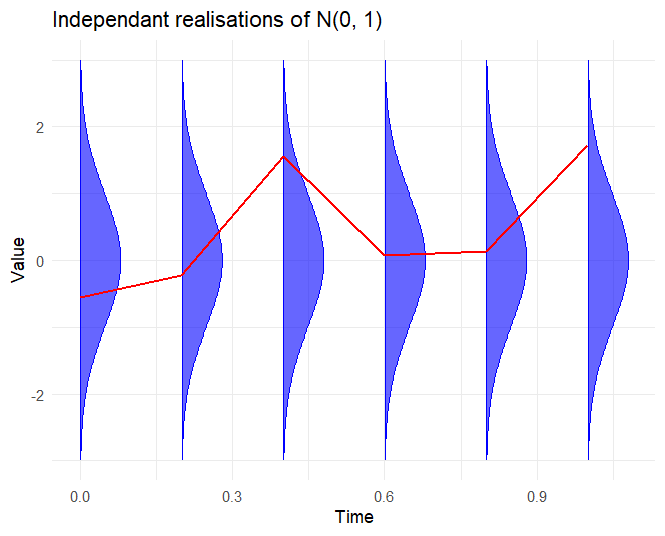
\includegraphics[width=\textwidth]{images/bb_without_cov.png}
    \caption{Folge von Normalverteilten Zufallsvariablen ohne Kovarianz}
    \label{fig:bb_without_cov}

    \centering
    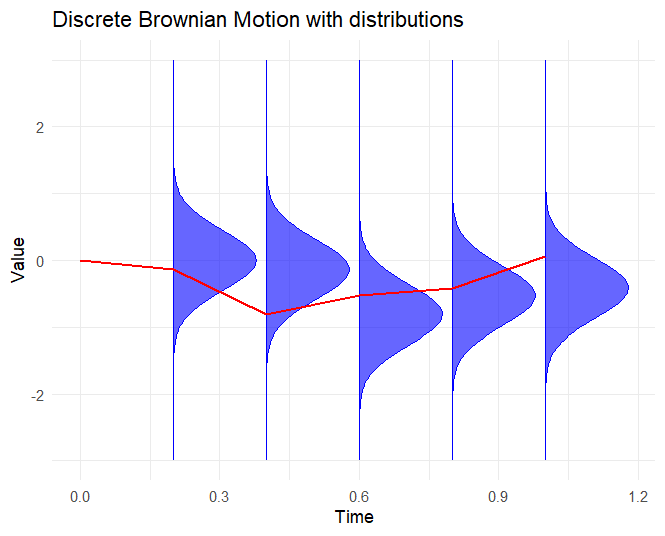
\includegraphics[width=\textwidth]{images/bb_with_cov.png}
    \caption{Visualierung der Verteilung der diskreten Brownschen Bewegung unter Beachtung der Kovarianzstruktur}
    \label{fig:bb_with_cov}

\end{figure}
\end{bem}

\begin{satz}[Selbstähnlichkeit und bedingte Verteilung der Brownschen Bewegung]
Für jedes $c > 0$ gilt
$$
W_{ct}(\omega) \overset{d}{=} \sqrt{c}\, W_t(\omega) \quad \text{für alle } t \ge 0,
$$
für alle $s < t$ gilt
$$
W_t - W_s \sim N(0, t-s),
$$
und die bedingte Verteilung von $W_t$ gegeben $W_s$ ist
$$
W_t \mid W_s \sim N\big(W_s, t-s\big).
$$
\textit{Beweis der ersten Behauptung (Selbstähnlichkeit).} \\
Für $t \ge 0$ gilt $W_{ct} \sim N(0, ct)$ und $W_t \sim N(0, t)$. Somit gilt
$$
\sqrt{c}\, W_t \sim N(0, c t).
$$
Da beide Normalverteilungen denselben Mittelwert $0$ und dieselbe Varianz $ct$ haben, folgt
$$
W_{ct} \stackrel{d}{=} \sqrt{c}\, W_t \quad \text{für jedes } t \ge 0.
$$  
\qed  \\
\textit{Beweis der zweiten Behauptung (Inkremente).} \\
Für $s < t$ gilt
$$
W_t - W_s = \lim_{N \to \infty} \big( b^{(N)}(t) - b^{(N)}(s) \big),
$$
wobei $b^{(N)}$ diskrete Approximierungen sind. Jedes Inkrement $b^{(N)}(t) - b^{(N)}(s)$ ist normalverteilt mit Erwartungswert $0$ und Varianz $t-s$. Durch Grenzwertbildung folgt
$$
W_t - W_s \sim N(0, t-s).
$$
\qed  \\
\textit{Beweis der dritten Behauptung (Bedingte Verteilung).} \\
Betrachte $(W_s, W_t)^T$, das multivariat normal verteilt ist mit
$$
E(W_s) = E(W_t) = 0, \quad
\mathrm{Cov}(W_s, W_t) = \min(s, t) = s.
$$  
Die Kovarianzmatrix lautet somit
$$
\Sigma = \begin{pmatrix} s & s \\ s & t \end{pmatrix}.
$$
Für die bedingte Verteilung ergibt die Standardformel der multivariaten Normalverteilung
$$
\begin{aligned}
E(W_t \mid W_s) &= E(W_t) + \mathrm{Cov}(W_t, W_s)\,V(W_s)^{-1} (W_s - E(W_s)) \\
&= 0 + \frac{s}{s} W_s = W_s, \\
V(W_t \mid W_s) &= V(W_t) - \frac{\mathrm{Cov}(W_t, W_s)^2}{V(W_s)} \\
&= t - \frac{s^2}{s} = t - s.
\end{aligned}
$$
Insgesamt folgt
$$
W_t \mid W_s \sim N(W_s,\, t-s).
$$ \qed
\end{satz}

\begin{korr}[Martingal-Eigenschaft der Brownschen Bewegung]
Die Brownsche Bewegung $W_t$ ist ein Martingal.
\textit{Beweis.} Aus dem vorigen Satz folgt
$$
E(W_t | W_s = v) = v.
$$
Damit ist $W_t$ ein Martingal. \qed
\end{korr}  

\begin{satz}[Stetigkeit der Pfade]
Der Pfad $t \mapsto W_t(\omega)$ ist fast sicher stetig.
\textit{Beweis.}
Für den Beweis wird eine neue Funktionen-Folge $\hat W_t^{(n)}(\omega), n \in \Bbb N$
definiert, wobei $\hat W_t^{(n)}(\omega)$ die lineare Interpolation der Werte $W_{k/2^n}(\omega), k=0,1,2,\ldots$ ist. 
Ohne Beschränkung der Allgemeinheit wird das Intervall $[0,1]$ betrachtet. Für $n \in \Bbb N$ und $k=0,\dots,2^n-1$ setze
$$I_{n,k}:=\big[k2^{-n},(k+1)2^{-n}\big].$$
Da die $I_{n,k}$ eine Zerlegung von $[0,1]$ bilden, ist
$$
\begin{aligned}
M_n &:=\sup_{t\in[0,1]}\big|\hat W^{(n+1)}_t-\hat W^{(n)}_t\big| 
\\ &= \max_{0\le k<2^n} \sup_{t\in I_{n,k}} \big|\hat W^{(n+1)}_t-\hat W^{(n)}_t\big| =\max_{0\le k<2^n}|Z_{n,k}|
\end{aligned}
$$
Für die unabhängigen Inkremente $Z_{n,k}$ mit
$$
Z_{n,k}\sim N\!\big(0,2^{-(n+2)}\big).
$$
Für eine Normalverteilung $Z\sim N(0,\sigma^2)$ und jedes $\varepsilon>0$ gilt (siehe z. B. Boucheron 2013 \cite{boucheron_concentration_2013} S. 2)
$$
P(|Z|>\varepsilon) \le 2\exp\!\Big(-\frac{\varepsilon^2}{2\sigma^2}\Big).
$$
Mit der Vereinigungsschranke folgt damit
$$
P(M_n>\varepsilon) \le \sum_{k=0}^{2^n-1} P(|Z_{n,k}|>\varepsilon)
\le 2^n\cdot 2\exp\!\Big(-\frac{\varepsilon^2}{2\sigma_n^2}\Big)
= 2^{\,n+1}\exp\!\Big(-\frac{\varepsilon^2}{2\sigma_n^2}\Big).
$$
Man wählt nun eine spezifische Folge $\varepsilon_n$ so, dass sich aus der rechten Seite eine geometrische Reihe ergibt. Setze
$$
\varepsilon_n := \sqrt{2(n+1)}\,\sigma_n.
$$
Dann gilt
$$
\frac{\varepsilon_n^2}{2\sigma_n^2}=n+1,
$$
und damit
$$
P(M_n>\varepsilon_n)\le 2^{\,n+1} e^{-(n+1)} = \big(2e^{-1}\big)^{\,n+1}.
$$
Da $2e^{-1}<1$ ist, ist die Folge auf der rechten Seite geometrisch und insbesondere summierbar. Folglich
$$
\sum_{n=1}^\infty P(M_n>\varepsilon_n) < \infty.
$$
Nach dem Reihenkriterium für fast sichere Konvergenz folgt, dass $M_n\to 0$ fast sicher.
Für $m \gt n \ge N$ beliebig gilt
$$\sup_{t}|\hat W^{(m)}_t - \hat W^{(n)}_t| \leq \sum_{k=n}^{m-1} M_k. \underset{N \to \infty} \longrightarrow 0$$
Weil jedes $\big(\hat W^{(n)}\big)_{n\in\Bbb N}$ eine stückweise lineare Funktion ist, folgt
dass $\big(\hat W^{(n)}\big)_{n\in\Bbb N}$ fast sicher eine Cauchy-Folge in $\Vert \cdot \Vert_{\infty}$ ist.
$\big(\hat W^{(n)}\big)_{n\in\Bbb N}$ konvergiert also gleichmäßig gegen den Grenzpfad $\widetilde W$, der stetig ist. \qed

Achtung: Es wurde nicht gezeigt, der Prozess $W_t^{(n)} \longrightarrow W_t$ gleichmäßig konvergiert. Für eine beliebige aber feste Realisierung
$t \mapsto W_t(\omega)$ wurde eine (reellwertige) Folge von stetigen Funktionen konstruiert, die gegen $t \mapsto W_t$ gleichmäßig konvergiert.
Da es sich um eine Folge stetiger Funktionen handelt, gilt die Stetigkeit unter gleichmäßiger Konvergenz auch gegen die Grenzfunktion $t \mapsto W_t$.
\end{satz}